\section*{Task 2: Linear Classification}
\subsection*{2a)} 
In the following we focus on the case of two classes $C_1$ and $C_2$ to keep the arguments simple. Our main goal is to compute 
\begin{align*}
p(C_1 | x) \text{ and } p(C_2 | x)
\end{align*}
such that we can decide to which class a data point $x$ belongs. Hence we classify $x$ into the class with the larger posterior probability. A discriminative model (e.g. logistic regression) tries to model these posterior probability directly. A generative model uses the Bayes rule to compute the posterior distribution after modelling first the joint probability distributions $p(x, C_1)$ and $p(x, C_2)$. We get:
\begin{align}
p(C_i|x) &= \frac{p(x|C_i)p(C_i)}{p(x)}  \\
&= \frac{p(x|C_i)p(C_i)}{p(x|C_1)p(C_1) + p(x|C_2)p(C_2)} \\
& = \frac{p(x,C_i)}{p(x, C_1) + p(x, C_2)}
\end{align}

The generative approach gives more information about the distribution such that we can sample new data points from the modelled distribution. This is not possible for the discriminative approach. \\
Many people argue that discriminative approaches are better, because we do not need to solve a more general problem in this case. We can directly compute the posterior probability. Furthermore we have many tricks to improve the discriminative approaches in practice. E.g. for logistic regression we can shrink parameters or impose margin constraints. Ng points out, that in theoretical settings we observe two phenomena. Logistic regression always has a lower asymptotic error than naive Bayes. But the error of naive Bayes decreases faster in the beginning. Hence if we have only few data points it may be better to use naive Bayes instead of logistic regression. However, after a certain amount of data, the logistic error will become lower and also stay lower than the error of naive Bayes. 
Information from [Ng 2001].
\subsection*{2b)}
In this exercise we use Fisher's Linear Discriminant to separate 3 classes. After observing the data we decided to use pairwise Fisher's Linear Discriminant for 2 classes ('one-vs-one'). That means that we separate $C_1$ and $C_2$ by $L_{12}$, then separate $C_1$ and $C_3$ by $L_{13}$ and finally separate $C_2$ and $C_3$ by $L_{23}$. $L_{ij}$ is the Fisher's Linear Discriminant Algorithm for classes $C_i$ and $C_j$. More precisely, we first used Fisher's discriminant approach to project each point to a one-dimensional subspace and then we used Bayesian Decision Theory (assuming a Gaussian distribution after projecting) to decide for $C_i$ or $C_j$. By majority vote on the three results, we then assigned $x$ to a class. 
\\
Out of 137 points in total we misclassified 19. One point from class 1 (red) was misclassified as being class 2 (yellow). 11 points from class 3 (green) were misclassified as being class 2 (yellow). 7 points from class 2 (yellow) were misclassified as being class 3 (green). If we look at the plot we can easily see that it is very hard to separate classes 2 and 3 with a straight line.  Further, red and yellow resp. red and green can be separated easily.  \\
In our example this method worked well but the intersection of the three linear classifiers will produce a triangle somewhere in the middle of the plot. This will cause problems if we want to classify points in it as our majority vote will not work there. But none of the points of the data set lay in this triangle. 
\begin{figure}
	\centering
	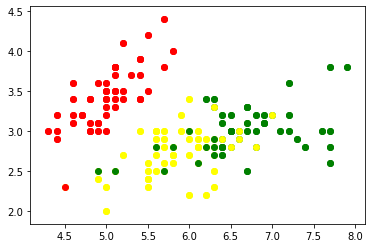
\includegraphics{Figure_2b_orig.png}
	\caption{The plot of the three classes with their original labels. Red: Class 1, Yellow: Class 2, Green: Class 3.}
	\label{fig:2b-Plot1}
\end{figure} 
\begin{figure}
	\centering
	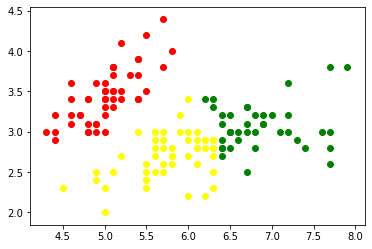
\includegraphics{Figure_2b_LDA.png}
	\caption{The plot of the three classes with the labels coming from $L_{12}$, $L_{13}$ and $L_{23}$. Red: Class 1, Yellow: Class 2, Green: Class 3.}
	\label{fig:2b-Plot2}
\end{figure} 
\\
Code Snippets for Task 2:
\begin{lstlisting}
def biased_ml_estimate(X):
    # mu
    mu = 0
    n = len(X)
    for i in range(n):
        mu = mu + X[i]
    mu = mu / n
    
    variance = 0
    for p in range(n):
        variance = variance + (X[p] - mu)**2
    variance = variance / (n-1) #for biased estimate divide by n
    return mu, variance

def gaussian_density_function(mu, sigma, x):
    c1 = 1 / np.sqrt(2*np.pi * sigma)
    c2 = np.exp(-0.5 * (x - mu)**2/ sigma)
    y = c1 * c2
    return y    

def compute_prior_probabilities(c1,c2):
    length_c1 = len(c1)
    length_c2 = len(c2)
    
    prob_c1 = length_c1 / (length_c1 + length_c2)
    prob_c2 = length_c2 / (length_c1 + length_c2)
    
    return(prob_c1, prob_c2)
    
def S_W_inverse(C_1, C_2):
    n_1 = len(C_1)
    n_2 = len(C_2)
    
    m_1 = np.mean(C_1, axis=0)
    m_2 = np.mean(C_2, axis=0)
    

    for i in range(n_1):
        if i == 0:
            sum_1 = np.outer(C_1[i] - m_1,C_1[i] - m_1)
        else:
            sum_1 = np.add(sum_1, np.outer(C_1[i] - m_1,C_1[i] - m_1))
    
    for i in range(n_2):
        if i == 0:
            sum_2 = np.outer(C_2[i] - m_2,C_2[i] - m_2)
        else:
            sum_2 = np.add(sum_2, np.outer(C_2[i] - m_2,C_2[i] - m_2))
    invers = np.linalg.inv(np.add(sum_1, sum_2))
    
    return invers

def fisher_linear_discriminant(C_1,C_2):
    S_W_inv = S_W_inverse(C_1, C_2)
    
    diff = np.mean(C_1, axis=0)-np.mean(C_2, axis=0)
    
    w = np.matmul(S_W_inv, diff)
    
    proj_C_1 = np.matmul(C_1, w)
    proj_C_2 = np.matmul(C_2, w)
    
    prob_c_1, prob_c_2 = compute_prior_probabilities(proj_C_1, proj_C_2)
    
    mu_1, variance_1 = biased_ml_estimate(proj_C_1)
    
    mu_2, variance_2 = biased_ml_estimate(proj_C_2)
    
    return w, mu_1, variance_1, mu_2, variance_2, prob_c_1, prob_c_2

def decision_function(w, mu_1, variance_1, mu_2, variance_2, prob_C_1, prob_C_2, x):
    proj_x = np.matmul(w,x)
    gauss_1 = gaussian_density_function(mu_1, variance_1, proj_x)
    gauss_2 = gaussian_density_function(mu_2, variance_2, proj_x)
    
    if (gauss_1/gauss_2) > (prob_C_2/prob_C_1):
        print("Point is classified in Class 1:", x)
    else:
        print("Point is classified in Class 2:", x)
    


if __name__ == "__main__":
    # 2a
    #Class 1 / Class 2
    onetwo_w, onetwo_mu_1, onetwo_variance_1, onetwo_mu_2, onetwo_variance_2, onetwo_prob_C_1, onetwo_prob_C_2 = fisher_linear_discriminant(dataset_1, dataset_2)
    print("Class 1 / Class 2 - w:",onetwo_w)
    
    #Class 2 / Class 3
    twothree_w, twothree_mu_2, twothree_variance_2, twothree_mu_3, twothree_variance_3, twothree_prob_C_2, twothree_prob_C_3 = fisher_linear_discriminant(dataset_2, dataset_3)
    print("Class 2 / Class 3 - w:",twothree_w)
    
    #Class 1 / Class 3
    onethree_w, onethree_mu_1, onethree_variance_1, onethree_mu_3, onethree_variance_3, onethree_prob_C_1, onethree_prob_C_3 = fisher_linear_discriminant(dataset_1, dataset_3)
    print("Class 1 / Class 3 - w:",onethree_w)
    
    counter = 0
    
    for x in ldaData:
        i = 0
        c1 = 0
        c2 = 0 
        c3 = 0
        
        # 12
        proj_x = np.matmul(onetwo_w,x)
        gauss_1 = gaussian_density_function(onetwo_mu_1, onetwo_variance_1, proj_x)
        gauss_2 = gaussian_density_function(onetwo_mu_2, onetwo_variance_2, proj_x)
        
        if (gauss_1/gauss_2) > (onetwo_prob_C_2/onetwo_prob_C_1):
            c1 = c1 + 1
        else:
            c2 = c2 + 1
            
        #13
        proj_x = np.matmul(onethree_w,x)
        gauss_1 = gaussian_density_function(onethree_mu_1, onethree_variance_1, proj_x)
        gauss_2 = gaussian_density_function(onethree_mu_3, onethree_variance_3, proj_x)
        
        if (gauss_1/gauss_2) > (onethree_prob_C_3/onethree_prob_C_1):
            c1 = c1 + 1
        else:
            c3 = c3 + 1
            
        #23
        proj_x = np.matmul(twothree_w,x)
        gauss_1 = gaussian_density_function(twothree_mu_2, twothree_variance_2, proj_x)
        gauss_2 = gaussian_density_function(twothree_mu_3, twothree_variance_3, proj_x)
        
        if (gauss_1/gauss_2) > (twothree_prob_C_3/twothree_prob_C_2):
            c2 = c2 + 1
        else:
            c3 = c3 + 1
        
        if max(c1,c2,c3) == c1:
            plt.scatter(x[0], x[1], c="red")
            #print("Class 1, x:", x)
        elif max(c1,c2,c3) == c2:
            plt.scatter(x[0], x[1], c="yellow")
            #print("Class 2, x:", x)
        elif max(c1,c2,c3) == c3:
            plt.scatter(x[0], x[1], c="green")
            #print("Class 3, x:", x)
        i = i + 1
    
            
        
    plt.plot()
    # for x in C_1:
    #     decision_function(w, mu_1, variance_1, mu_2, variance_2, prob_C_1, prob_C_2, x)
        
    # for x in C_2:
    #     decision_function(w, mu_1, variance_1, mu_2, variance_2, prob_C_1, prob_C_2, x)
    
    plt.scatter(dataset_1[:,0],dataset_1[:,1], c="red")
    plt.scatter(dataset_2[:,0],dataset_2[:,1], c="yellow")
    plt.scatter(dataset_3[:,0],dataset_3[:,1], c="green")
\end{lstlisting}
\section*{References}
\begin{tabular}{lp{15cm}}
	$[Ng \text{ } 2001]$ & A. Y. Ng, M. I. Jordan, On Discriminative vs. Generative Classifiers: A
	Comparison of Logistic Regression and Naive Bayes, in: Proceedings
	of the 14th International Conference on Neural Information Processing
	Systems: Natural and Synthetic, NIPS’01, MIT Press, Cambridge, MA,
	USA, 2001, pp. 841–848.
\end{tabular}
